\documentclass{article}[18pt]
\usepackage{../../../../format}
\lhead{ToC - Models of Computation}
\usepackage{mathrsfs}



\begin{document}
\begin{center}
\underline{\huge Turing Machines}
\end{center}
A turing machines has an infinite tape (memory). There is a finite-state "program" that controls a tape head. The head can read, write and move around (in both directions) on the tape.\\
\\
A typical program instructions: if the finite control is in state $p$ and the head reads $b$, then write $a$, move the head to the left and go to state $q$
\section{Formal Definition of TM}
A Turing Machine is a 7-tuple $(Q,\Sigma, \Gamma,\delta,q_0,q_{accept},q_{reject})$
\begin{enumerate}
	\item Q is the set of states
	\item $\Sigma$ is the input alphabet not containing the special \textbf{blank} symbol $\sqcup$
	\item $\Gamma$ is the tape alphabet satisfying $\Sigma \subset \Gamma$ and $\sqcup \in \Gamma$
	\item $\delta: Q\times \Gamma \rightarrow Q \times \Gamma \times \{L,R\}$ is the transition function (If in Q moving to $\Gamma$, replace the state and move the head to the \textbf{L}eft or \textbf{R}ight).This is deterministic
	\item $q_0\in Q$ is the start state
	\item $q_{accept} \in Q$ is the accept state, and
	\item $q_{reject}\in Q$ is the reject state $q_{accept}\neq q_{accept}$
\end{enumerate}
\subsection{Added notes}
The first $\sqcup$ denotes the start of the blanks
\section{Computation of TM}
The tape content is unbounded but always \textbf{finite}; the first (leftmost) blank marks the end of the tape content\\
\\
A configuration consists of three items: the current state, the tape content and the head location\\
\\
The configuration $C_1$ yields the configuration $C_2$ if the TM can legally go from $C_1$ to $C_2$ in a single step (using the transition function once)\\
\\
The start configuration on an input $w\in \Sigma^*$ consists of the start state $q_0,w$ as the tape content, and the head location being the first (leftmost) position of the tape\\
\\
An accepting (rejecting) configuration is a configuration whose state is $q_{accept}$ ($q_{reject}$,respectively). Accepting and rejecting configurations are halting configurations.\\
\\
\\
A TM $\mathscr{M}$ accepts an input $w$ if there is a sequence of configurations $C_1,C_2,...,C_k$ such that
\begin{enumerate}
	\item $C_1$ is the start configuration of $\mathscr{M}$ on input $w$
	\item $C_i$ yields $C_{i+1}$ for $1\leqslant i\leqslant k-1$, and
	\item $C_k$ is an accepting configuration
\end{enumerate}
The set of string accepted by $\mathscr{M}$ constitutes the language of $\mathscr{M}$, denoted by $L(\mathscr{M})$
\subsection{Example}
He did example 3.7 from theory of computation.\\
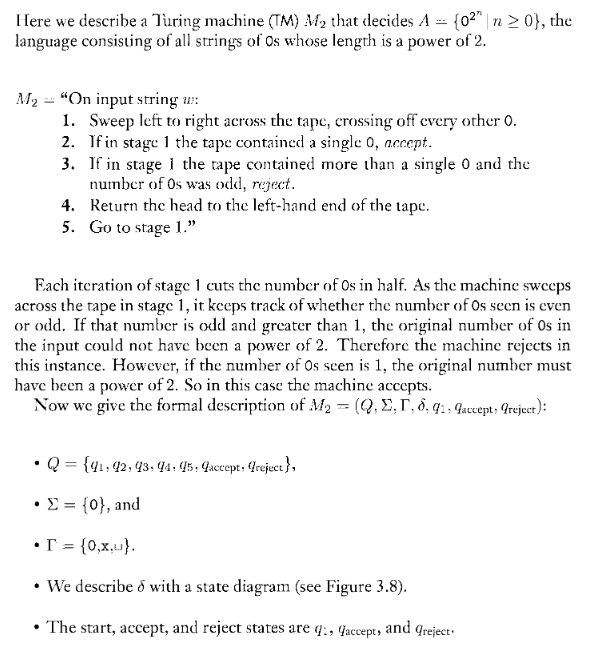
\includegraphics[scale=0.7]{Example}

\section{Turing-Recognisable and Turing-Decidable languages}
\textbf{Definition 1} - A language $\mathscr{L}$ is Turing-Recognisable, if there is a TM $\mathscr{M}$ that recognises it, i.e. $\mathscr{L}=L(\mathscr{M})$\\
\textbf{Definition 2} - A language $\mathscr{L}$ is Turing-Decidable, if there is a TM $\mathscr{M}$ that accepts every $w\in\mathscr{L}$ and reject every $w\notin \mathscr{L}$\\
\\
\textbf{Important note 1}: If $\mathscr{M}$ recognises $\mathscr{L}$, it may or may not halt on words not in $\mathscr{L}$. However, if $\mathscr{M}$ decides $\mathscr{L}$, it always halts\\
\textbf{Important note 2}: The standard terminology is "r.e." (stands for recursively enumerable) instead of "Turing-Recognisable" and "recursive" instead of "Turing-Decidable"
\section{Multitape TM}
A Multitape TM is an ordinary (single tape) TM with several tapes, each of them having its own head. The only difference in the formal definition is the transition function, which is now
$$\delta: Q \times \Gamma^{k} \rightarrow Q \times \Gamma^{k} \times\{L, R\}^{k}$$
where $k$ is the number of tapes.\\
\\
\textbf{Theorem.} - Every Multitape TM has an equivalent single tape TM\\
\\
Put the encoding from each turing machine in sequence, with a special character to act as a separator between each encoding so that the turing machine knows to jump.\\
\\
Add $\dot{a},\dot{b}...$ for all the characters in the language, denote the position of the head in the original machine.\\
\\
A single step in the multi tape TM will take many steps in a single tape TM, up to the total length of all the chunks added together.
\section{Non-deterministic TM}
A non-deterministic TM has a transition function
$$\delta: Q \times \Gamma \rightarrow \mathscr{P}(Q \times \Gamma \times\{L, R\})$$
This transition function creates the power set of all options, including the empty set.\\
\\
\textbf{Theorem} - Every Non-deterministic TM has an equivalent deterministic TM\\
\\
\textbf{Proof. Idea:} Consider the tree of all possible computations of the Non-deterministic TM. Start from the root (the start configuration) and do a breadth-first search.  Accept only if an accepting configuration is found. Note that:
\begin{enumerate}
	\item Depth First Search would not work - might go down forever
	\item Can use a multitape TM to implement the breadth-first search
\end{enumerate}
\section{Enumerators}
The concept of an "enumerator" is important as it justifies the term recursively enumerable.\\
\\
A language $\mathscr{L}$ is enumerated by a TM $\mathscr{M}$ if $\mathscr{M}$ starts on an empty input and outputs a (potentially infinite) list of words that contains every word in $\mathscr{L}$ and nothing else\\
\\
\textbf{Theorem} - A language is R.E iff some enumerator enumerates it
\section{Church-Turing Thesis}
The intuitive notion of algorithm is equivalent to the mathematical concept of algorithm defined by Turing Machines (or any other formal model of computation)
\section{Universal Turing Machine}
\textbf{Proposition} - Every TM $\mathscr{M}$ can be encoded as a word over a finite alphabet, We shall use $\langle\mathscr{M}\rangle$ to denote the encoding of a Turing machine $\mathscr{M}$\\
\textbf{Theorem} - There is a TM $\mathscr{U}$ that takes a two-part input, the encoding of a TM $\mathscr{M},\langle\mathscr{M}\rangle$, and a word $w$, and simulate $\mathscr{M}$ on $w$. $\mathscr{U}$ is called a universal turing machine.
\section{The Halting Problem}
\textbf{The Halting Problem}: Given a (encoding of a) TM $\mathscr{M}$, and a word $w$, does $\mathscr{M}$ terminate on $w$?\\
\textbf{Proposition}: The Halting Problem is Turing-recognisable\\
\textbf{Proof}: Run a Universal TM on the pair $(\langle\mathscr{M}\rangle,w)$. Accept if the computation eventually terminates.\\
\textbf{Proposition}: The halting problem is not turing-decidable\\
\\
\textbf{Proof}: Assume for contradiction that there is a TM $\mathscr{H}$ that decides the halting problem
$$\mathscr{H}(\langle\mathscr{M}\rangle, w)=\left\{\begin{array}{ll}{\operatorname{accept}} & {\text { if } \mathscr{M} \text { terminates on } w} \\ {\text { reject }} & {\text { if } \mathscr{M} \text { does not terminate on } w}\end{array}\right.$$
Consider the TM $\mathscr{D}$ that takes a TM $\mathscr{M}$ as an input does the following:
$$\mathscr{D}(\langle\mathscr{M}\rangle)=\left\{\begin{array}{ll}{\operatorname{accept}} & {\text { if } \mathscr{H}(\langle\mathscr{M}\rangle,\langle\mathscr{M}\rangle) \text { rejects }} \\ {\operatorname{loop}} & {\text { if } \mathscr{H}(\langle\mathscr{M}\rangle,\langle\mathscr{M}\rangle) \text { accepts }}\end{array}\right.$$
What happens when $\mathscr{D}$ runs on its own encoding $\langle D\rangle$?! There are two possibilities:
\begin{enumerate}
	\item $\mathscr{D}$ terminates on $\langle D \rangle$. By the construction of $\mathscr{D}$, we have that $\mathscr{H}(\langle D\rangle, \langle D \rangle)$ rejects, and by the definition of $\mathscr{H}$, it follows that $\mathscr{D}$ does not terminate on $\langle D \rangle$
	\item $\mathscr{D}$ does not terminate on $\mathscr{D}$. By the construction of $\mathscr{D}$, we have that $\mathscr{H}(\langle D\rangle, \langle D \rangle)$ accepts, and by the definition of $\mathscr{H}$, it follows that $\mathscr{D}$ terminates on $\langle \mathscr{D}\rangle$ 
\end{enumerate}
\section{Turing-Recognisable vs Turing-Decidable}
\textbf{Theorem}: A language $\mathscr{L}$ is Turing-Decidable iff both $\mathscr{L}$ and its complement $\overline{\mathscr{L}}$ are Turing-recognisable\\
\\
\textbf{Proof (of the "interesting" direction only)}: Suppose $\mathscr{M}_1$ recognises $\mathscr{L}$ and $\mathscr{M}_2$ recognises $\overline{\mathscr{L}}$. On an input $w$, run $\mathscr{M}_1$ and $\mathscr{M}_2$ "in parallel" (i.e. simulate alternating steps of $\mathscr{M}_1$ and $\mathscr{M}_2$ on a multitape TM). Either $\mathscr{M}_1$ or $\mathscr{M}_2$ must eventually accept; accept it if $\mathscr{M}_1$ accepts and reject it is $\mathscr{M}_2$ accepts
\section{Context Sensitive Languages}
\textbf{Definition}: A Linear Bounded Automaton (LBA) is a non-deterministic single-tape TM that can use only the part of the tape on which the input is initially written.\\
\textbf{Definition}: A language is context-sensitive if some LBA recognises it\\
\\
Examples of languages that are context-sensitive but not context-free
\[
\begin{array}{l}{\left\{a^{n} b^{n} c^{n} | n \in \mathbb{N}\right\}} \\ {\left\{w w | w \in\{0,1\}^{*}\right\}}\end{array}
\]
\section{Chomsky Hierarchy}
\begin{enumerate}
	\item \textbf{Regular}: Rules of the form $U\rightarrow aV$ or $U\rightarrow a$, where U and V are variables and a is either a terminal of $\epsilon$
	\item \textbf{Context-Free}: Rules of the form $U\rightarrow s$, where u is a variable and $s$ is any string of variables and terminals
	\item \textbf{Context-Sensitive}: Rules of the form $t\rightarrow s$, where $t,s $ are string of variables and terminals, $t$ contains at least one variable and $|t|\leqslant |s|$
	\item \textbf{General (Turing-recognisable)}: rules of the form $t\rightarrow s$, where $t, s$ are string of variables and terminals and $t$ contains at least one variable
\end{enumerate}
\subsection{Example $a^nb^nc^n$}
\[
\begin{aligned} S & \rightarrow a S B C \\ S & \rightarrow \varepsilon \\ C B & \rightarrow B C \\ a B & \rightarrow a b \\ b B & \rightarrow b b \\ b C & \rightarrow b c \\ c C & \rightarrow c c \end{aligned}
\]
\section{Real world}
\begin{enumerate}
	\item \textbf{Regular}: (advanced) text search of regular expressions (grep), lexical analysers (lex)
	\item \textbf{Context-Free}: the syntax of programming languages, i.e. (yacc, bison)
	\item \textbf{Context-Sensitive}: none?
	\item \textbf{General (Turing-recognisable)}: everything a computer can do
\end{enumerate}

\end{document}